\documentclass[11pt, oneside]{article} 
\usepackage{geometry}
\geometry{letterpaper} 
\usepackage{graphicx}
	
\usepackage{amssymb}
\usepackage{amsmath}
\usepackage{parskip}
\usepackage{color}
\usepackage{hyperref}

\graphicspath{{/Users/telliott_admin/Dropbox/Tex/png/}}
% \begin{center} 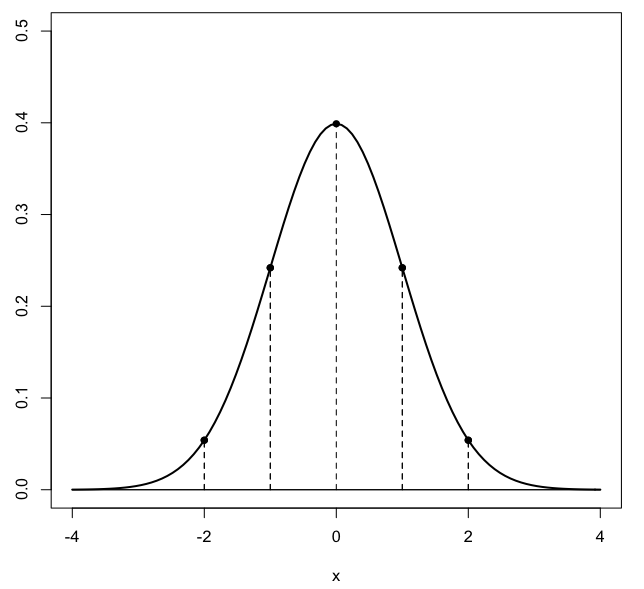
\includegraphics [scale=0.4] {gauss3.png} \end{center}

\title{e is irrational}
\date{}

\begin{document}
\maketitle
\Large
I assume you know about $e$.  I found a beautiful proof of the irrationality of $e$ in the calculus text by Courant and Robbins.

The proof is by contradiction.  We start by assuming that $e$ is rational.
\[ e = \frac{p}{q}, \ \  p,q \in \mathbb{N} \]

We make use of the infinite series representation of $e$
\[ e = 1 + 1 + \frac{1}{2!}  + \frac{1}{3!} + \frac{1}{4!} + \cdots \]

From this, it is obvious that $e > 2$.  

We can also prove that $e < 3$ since
\[ \frac{1}{2!}  + \frac{1}{3!} + \frac{1}{4!} + \cdots = \frac{1}{2}  + \frac{1}{6} + \frac{1}{24} + \cdots \]
and
\[ \frac{1}{2}  + \frac{1}{6} + \frac{1}{24} + \cdots < \frac{1}{2} + \frac{1}{4} + \frac{1}{8} \cdots \]
since each term on the left is smaller than the corresponding term on the right, but we know that
\[ \frac{1}{2} + \frac{1}{4} + \frac{1}{8} \cdots = 1 \]

\newpage 

\textbf{Proof}:
\[ \frac{1}{2} + \frac{1}{4} + \frac{1}{8} \cdots = 1 \]


\includegraphics [scale=0.5] {series1.png}

Equating the series representation to the rational fraction $p/q$:
\[ \frac{p}{q} = 1 + 1 + \frac{1}{2!}  + \frac{1}{3!} + \frac{1}{4!} + \cdots \]
Multiply both sides by $q!$.  For the left-hand side, we have 
\[ e \ q! = \frac{p}{q} \ q! = p (q-1)! \]

Clearly, the left-hand side, $e\ q! = p (q-1)!$, is an integer.

Therefore, the right-hand side must also be an integer.  We have the series
\[ q! + q! + \frac{q!}{2!}  + \frac{q!}{3!}  + \cdots + \frac{q!}{(q-1)!} + \frac{q!}{q!} + \frac{q!}{(q+1)!} + \cdots \]
Now, 
$q!$ is obviously an integer. And for every integer $k < q$, $k!$ divides $q!$ evenly 
\[ \frac{q!}{k!} = q \times (q-1) \times (q-2) \cdots \times (q-k+1) \]
In our series
\[ q! + q! + \frac{q!}{2!}  + \frac{q!}{3!}  + \cdots + \frac{q!}{(q-1)!} + \frac{q!}{q!} + \frac{q!}{(q+1)!} + \cdots \]
all the terms to the left of $q!/(q-1)!$ are integers, as is $q!/(q-1)! = q$ and $q!/q! = 1$.  
\vspace{2 mm}

So now our only concern is with the fractions that follow.  We will show that these sum up to something less than $1$.  We have
\[ \frac{1}{(q+1)} + \frac{1}{(q+1)(q+2)} + \frac{1}{(q+1)(q+2)(q+3)} + \cdots \]

Since $q$ is an integer and $q >= 2$
\[ \frac{1}{(q+1)} <= \frac{1}{3} \]
\[ \frac{1}{(q+1)(q+2)} <= (\frac{1}{3})^2 \]
and so on, and the entire remaining series of fractions is less than or equal to
\[ \frac{1}{3} + (\frac{1}{3})^2 + (\frac{1}{3})^3 + \cdots \]
This is the geometric series with $r = 1/3$ and first term equal to r, and we know the sum to be
\[ \frac{1}{3} ( 1 / (1-\frac{1}{3}) ) = \frac{1}{2} \]
Since the right-hand side is equal to an integer plus something less than or equal to $1/2$, it is not an integer, and cannot be equal to the left-hand side, which is an integer.  We have reached a contradiction.  Therefore $e$ cannot be equal to $p/q$, for $p,q \in \mathbb{N}$.


\end{document}